\chapter{Evaluation}
\label{ch:eval}

\section{Experimental Setup}\label{sec:experimental-setup}

\subsection{Testbed Configuration}\label{subsec:testbed-configuration}
We conducted our benchmarks on a Google Pixel 8 equipped with a Google Tensor G3 chip, comprising 1\,$\times$\,Cortex-X3 (2.91\,GHz), 4\,$\times$\,Cortex-A715 (2.37\,GHz), and 4\,$\times$\,Cortex-A510 (1.7\,GHz) cores, with Memory Tagging Extension (MTE) enabled.
To mitigate thermal throttling, we attached a cooling fan to the device.
Additionally, we pinned benchmarks to the low-power Cortex-A510 cores, which significantly decreased thermal throttling and noise in our benchmarks. \todo{should we leave this in?}
As of the date of writing, this is the sole commercially available device featuring MTE.

\begin{table}[ht]
    \centering
    \small
    \begin{tabular}{c || c c c}
        \hline
        \textbf{Variant} & \textbf{64-bit} & \textbf{memsafe} & \textbf{bounds-chk} \\
        \hline
        wasm32           & No              & No               & No                  \\
        wasm64           & Yes             & No               & No                  \\
        mem-safety       & Yes             & Yes              & No                  \\
        mte-bounds       & Yes             & No               & Yes                 \\
        all              & Yes             & Yes              & Yes                 \\
        \hline
    \end{tabular}
    \caption{Benchmarking Variants}
    \label{tab:benchmark-variants}
\end{table}

\subsection{Benchmark Variants}\label{subsec:benchmark-variants}
The benchmarks utilized were from the Polybench-C suite.
\todo{add more real-world benchmarks}
The variants compared are detailed in Table \ref{tab:benchmark-variants}.

\section{Performance Overheads}

\begin{figure*}[ht]
    \centering
    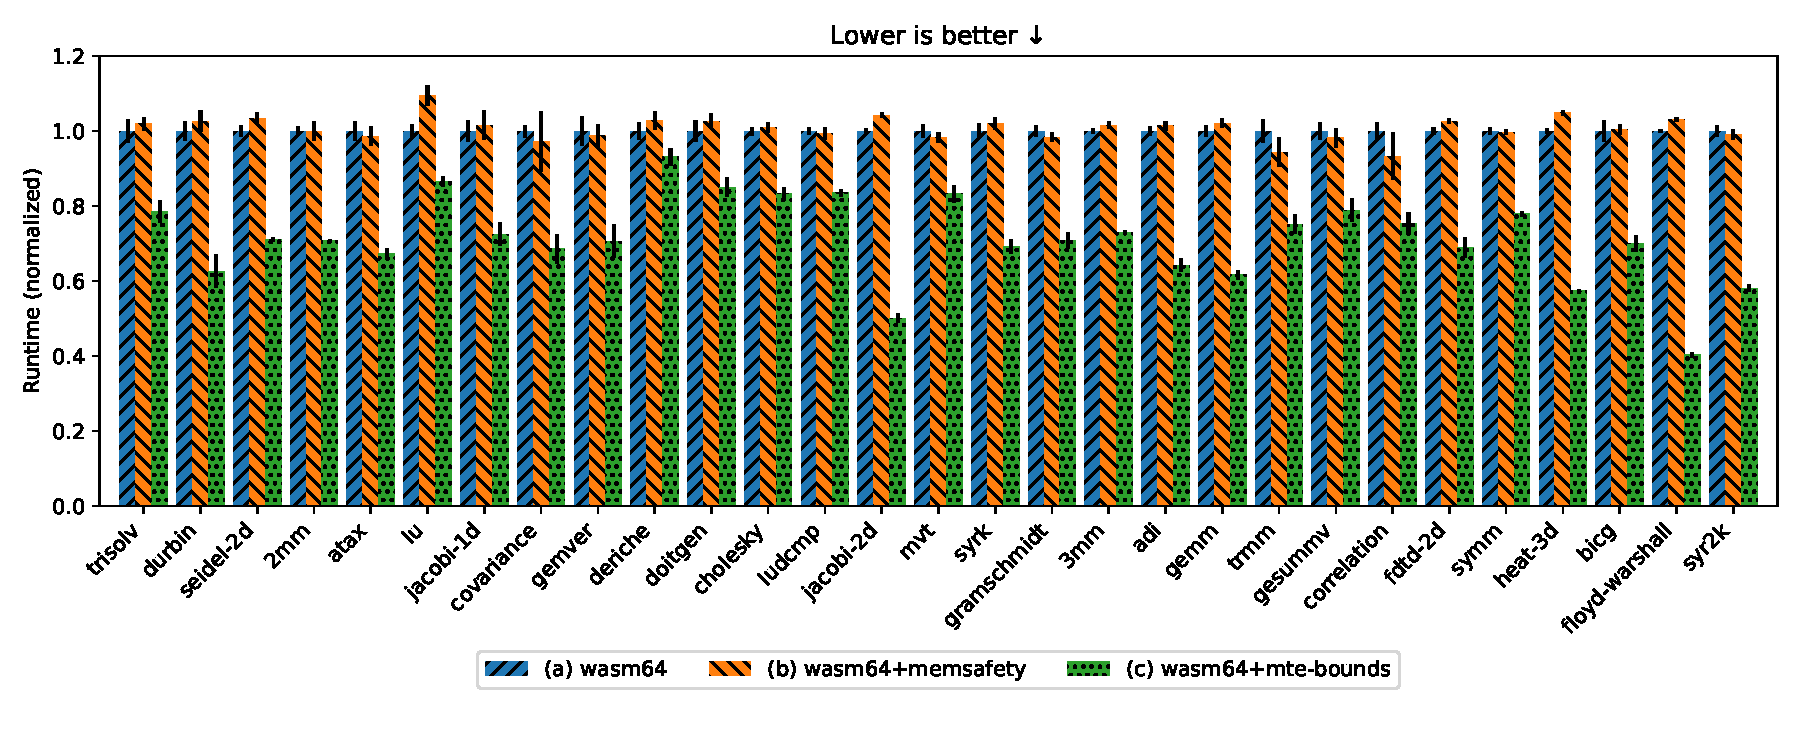
\includegraphics[width=\textwidth]{./plots/runtimes}
    \caption{{PolyBench-C runtime overheads of {\projectname{}}. (a) Baseline. (b) Relative overhead of wasm64 with memory safety features. (c) Bounds checks implemented using MTE.}{}}
    \label{fig:runtime_overheads}
\end{figure*}

Figure~\ref{fig:runtime_overheads} illustrates the runtime overheads for PolyBench-C benchmarks.
The mean runtime compared to the baseline for the memory safety implementation is 100.8\,\%, with a maximum of 109.4\%.
With memory safety features disabled, and MTE employed for bounds checking, we reach a median runtime of 70.9\% relative to the baseline, with minimum and maximum runtimes of 40.4\% and 93.1\%, respectively.

\todo{combining bounds + memsafe}

\section{Memory Overheads}\label{sec:memory-overheads}

\begin{figure*}[ht]
    \centering
    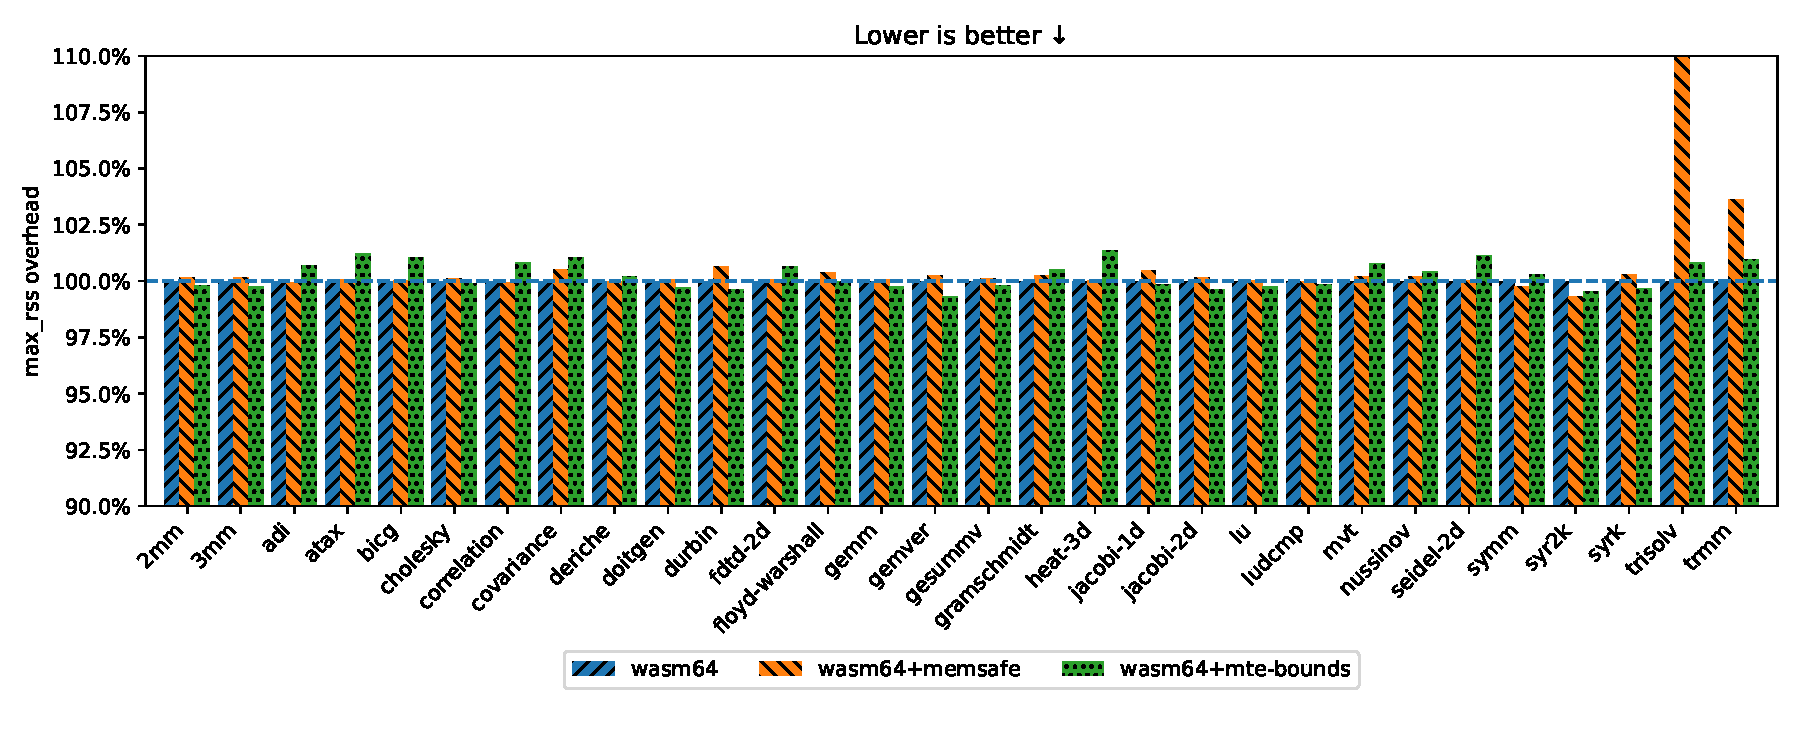
\includegraphics[width=\textwidth]{./plots/mem-overhead}
    \caption{{PolyBench-C memory overheads of {\projectname{}}. (a) Baseline. (b) Relative overhead of wasm64 with memory safety features. (c) Bounds checks implemented using MTE.}{}}
    \label{fig:memory_overheads}
\end{figure*}

We measure the memory overhead with GNU time.

Memory tagging incurs overhead, particularly for small allocations due to the 16-byte alignment required for MTE.
The MTE backend further introduces overhead, as observed in Figure \ref{fig:memory_overheads}, due to OS-level memory allocation requirements when MTE is active.
Enabling our memory safety mechanism results in an average overhead of 1\%, with a range of -0.67\% to 23.5\%.
In contrast, replacing bounds checks with MTE, which necessitates tagging the entire WebAssembly linear memory, leads to an average memory overhead of 0.26\%, with a range of -0.7\% to 1.4\%.

\section{Security Guarantees}\label{sec:security-guarantees}


\todo{insert evaluation here}

\section{Overhead of wasm32}
\label{sec:eval-wasm32-wasm64}

\todo{insert evaluation here}


